% Subsection on resistive divider

Pour changer le volume, on utilise un diviseur résistif. Une simple résistance variable, appelée aussi \emph{potentiomètre}, fait l'affaire. Une photo de potentiomètre se trouve à la Figure \ref{fig:potentiometre_pic}.\\

Un potentiomètre est un composant à 3 accès (à 3 pattes) qui possède une molette qui se tourne, par exemple avec un tournevis. Le schéma d'un potentiomètre est renseigné à la Figure \ref{fig:potentiometre_sch}. Entre les deux accès les plus éloignés $\alpha$ et $\gamma$, il y a une résistance fixe valant $R_{\alpha\gamma} = R_{\alpha\beta}+R_{\beta\gamma}$, de par exemple $1k\Omega$. L'unité de $1\Omega$ (ohm) correspond à une chute de tension de $1V$ (volt) lorsqu'un courant de $1A$ (ampère) traverse la résistance.\\

En tournant la molette dans un sens ou dans l'autre, l'on change les valeurs des résistances $R_{\alpha\beta}$ et $R_{\beta\gamma}$ (mais leur somme reste fixe). En prenant le noeud $\gamma$ comme référence (à la masse), la tension au noeud $\beta$ est une fraction de la tension du noeud $\alpha$ et peut être ajustée à la valeur désirée grâce à la molette. Dans le contexte du son, cela revient à contrôler son volume.\\

\begin{minipage}[c]{0.45\textwidth}
	\centering
	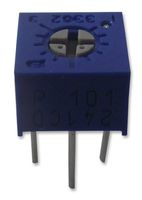
\includegraphics[width=0.4\textwidth]{figures/potentiometre_picture.jpg}
	\captionof{figure}{Schéma d'un potentiomètre.}
	\label{fig:potentiometre_pic}
\end{minipage}
\hfill
\begin{minipage}[c]{0.45\textwidth}
	\centering
	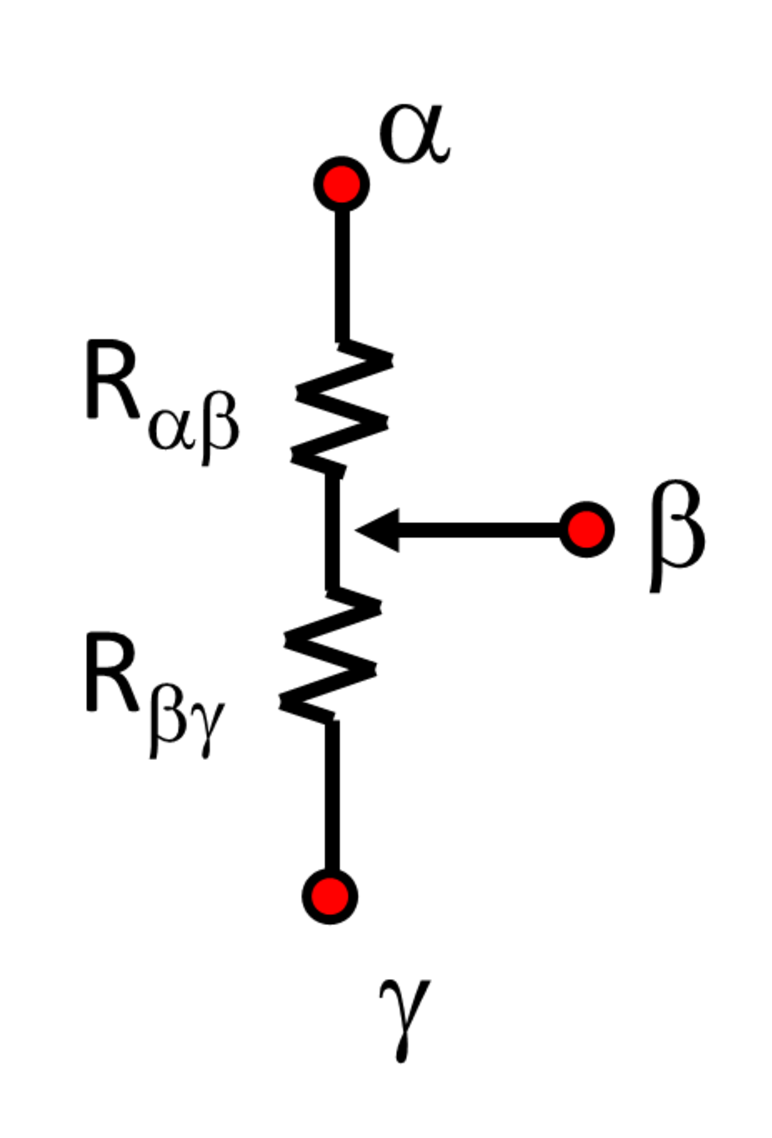
\includegraphics[width=0.4\textwidth]{figures/potentiometre.pdf}
	\captionof{figure}{Schéma d'un potentiomètre.}
	\label{fig:potentiometre_sch}
\end{minipage}
\vspace{1cm}